\documentclass[a4paper]{article}

%% Language and font encodings
\usepackage[english]{babel}
\usepackage[utf8x]{inputenc}
\usepackage[T1]{fontenc}

%% Sets page size and margins
\usepackage[a4paper,top=3cm,bottom=2cm,left=2cm,right=2cm,marginparwidth=2cm]{geometry}

%% Useful packages
\usepackage{amsmath}
\usepackage{amsfonts}
\usepackage{bbm}
\usepackage{graphicx}
\usepackage[colorinlistoftodos]{todonotes}
\usepackage[colorlinks=true, allcolors=blue]{hyperref}
\usepackage{float}
\usepackage{enumerate}
\usepackage[export]{adjustbox}
\usepackage{mathrsfs}
\usepackage{subcaption}

\usepackage{tikz}
\tikzset{
    vertex/.style={circle,draw,minimum size=1.5em},
    edge/.style={->,> = latex'}
}

\title{Stochastic Processes}
\author{Kevin Chang}

\graphicspath{ {./images/} }

\begin{document}
\maketitle

\section{Moment Generating Function}
\begin{itemize}
    \item Moment Generating Function: $\mathbb{E}[e^{tX}]$
        \begin{itemize}
            \item Property:
                \begin{itemize}
                    \item $\mathbb{E}[e^{tX}] = \int_{-\infty}^\infty e^{tx} f_X(x) dx$
                    \item $\mathbb{E}[e^{tX}] = \sum_{k=0}^\infty \mathit{E}[X^k] \frac{t^k}{k!}$
                        \begin{itemize}
                            \item $e^{tx} = \sum_{k=0}^\infty \frac{(tx)^k}{k!}$
                            \item $\mathit{E}[e^{tX}] = \mathit{E}[\sum_{k=0}^\infty \frac{(tX)^k}{k!}] = \sum_{k=0}^\infty \mathit{E}[X^k] \frac{t^k}{k!}$
                        \end{itemize}
                    \item $\frac{d\mathbb{E}[e^{tX}]}{dt} = \mathbb{E}[X]$
                    \item $\mathbb{E}[e^{t(aX+b)}] = e^tb\mathbb{E}[e^{taX}]$
                    \item Not all random variables have Moment generating function
                \end{itemize}
        \end{itemize}
    \item Characteristic Function: $\mathbb{E}[e^{itX}]$
        \begin{itemize}
            \item Property:
                \begin{itemize}
                    \item All random variables have Moment generating function
                \end{itemize}
        \end{itemize}
    \item Joint Moment Generating Function: $G(x, y) = \mathbb{E}[e^{xX}e^{yY}]$
    \item Property:
        \begin{itemize}
            \item (Joint) moment generating funciton uniquely determines the (joint) CDF
        \end{itemize}
    \item Example
        \begin{itemize}
            \item Trapped miner's random walk
                \begin{itemize}
                    \item Miner has probability of $\frac{1}{3}$ to waste 3 hours in vain, $\frac{1}{3}$ to waste 5 hours in vain, and $\frac{1}{3}$ to spend 2 hours to go out of the mine.
                    \item $X$ is the random variables of the hours to go out of the mine
                    \item $Y_i$ is the random variables of the hours for the $i$-th action.
                    \item $\mathbb{E}[e^{tX}] = \mathbb{E}[e^{tX}|Y_1 = 2] + \mathbb{E}[e^{tX}|Y_1 = 3] + \mathbb{E}[e^{tX}|Y_1 = 5]$

                        $= \mathbb{E}[e^{2t}] + \mathbb{E}[e^{t(X+3)}] + \mathbb{E}[e^{t(X+5)}]$
                    \item Find expectation and variance by joint moment generating function
                \end{itemize}
        \end{itemize}
\end{itemize}

\section{Expectation}
\begin{itemize}
    \item $N$ i.i.d. events, when $N$ is a random variable
        \begin{itemize}
            \item Suppose $N$ is a integer random variable
            \item Suppose $X_1, \dots, X_i, \dots, X_N$ are i.i.d random variables with mean $\mu$ and variance $\sigma^2$
            \item $Y = \sum_{i = 1}^N X_i$
            \item $\mathbb{E}[Y] = \mathbb{E}[N] \mu$
                \begin{itemize}
                    \item $\mathbb{E}[Y] = \sum_{n = 1}^\infty \mathbb{E}[\sum_{i = 1}^N X_i|N=n] P[N=n]$

                        $= \mu \times \sum_{n=1}^\infty n P[N=n] = \mathbb{E}[N] \mu$
                \end{itemize}
            \item $\mathbb{E}[Y^2] = \mathbb{E}[N] \mathbb{E}[X^2] + \mathbb{E}[N^2] \mu^2 - \mathbb{E}[N] \mu^2$
                \begin{itemize}
                    \item $\mathbb{E}[Y^2] = \sum_{n = 1}^\infty \mathbb{E}[(\sum_{i = 1}^N X_i)^2|N=n] P[N=n]$
                        $= \sum_{n = 1}^\infty (n \mathbb{E}[X_i^2] + n(n-1)\mu^2) P[N=n]$

                        $= \mathbb{E}[N] \mathbb{E}[X^2] + \mathbb{E}[N^2] \mu^2 - \mathbb{E}[N] \mu^2$
                \end{itemize}
            \item $\mathit{Var}(Y) = \mathbb{E}[N]\sigma^2 + \mathit{Var}(N)\mu^2$
        \end{itemize}
    \item Expectation by $P[X>x]$
        \begin{itemize}
            \item $\mathbb{E}[X] = \sum_x P[X > x]$, when $X$ is a non-negative discrete random variable
                \begin{itemize}
                    \item $\mathbb{E}[X] = \sum_{x=0}^\infty x P[X = x] = \sum_{x=0}^\infty \sum_{y=0}^{x-1} P[X = x] = \sum_{y=0}^\infty \sum_{x=y + 1}^\infty P[X = x] = \sum_{y = 0}^\infty P[X > y]$
                \end{itemize}
            \item $\mathbb{E}[X] = \int_0^\infty P[X > x] dx$, when $X$ is a non-negative continuous random variable
                \begin{itemize}
                    \item $\mathbb{E}[X] = \int_0^\infty x f_X(x) dx = \int_0^\infty \int_0^x f_X(x) dy dx = \int_0^\infty \int_y^\infty f_X(x) dx dy = \int_0^\infty P[X > y] dy$
                \end{itemize}
        \end{itemize}
\end{itemize}

\section{Inequality}
\begin{itemize}
    \item Markov Inequality

        Definition:
        \begin{itemize}
            \item Suppose $X \geq 0$, then $P[X \geq \epsilon] \leq \frac{\mathbb{E}[X]}{\epsilon}$
        \end{itemize}

        Proof:
        \begin{enumerate}
            \item $\mathbb{E}[X] = \int_0^\infty x f_X(x) \geq \int_\epsilon^\infty x f_X(x) \geq \epsilon \int_\epsilon^\infty f_X(x) = \epsilon P[X \geq \epsilon]$
            \item $X(\omega) \geq \epsilon \mathbbm{1}_{X(\omega) \geq \epsilon}, \forall \omega \in S$
                \begin{itemize}
                    \item Calculate expectation on both side.
                    \item $\mathbb{E}[X] \geq \epsilon P[X \geq \epsilon]$
                \end{itemize}
        \end{enumerate}
        Property:
        \begin{itemize}
            \item The equality happens when $P[X=k] = 0, \forall k \not \in \{0, \epsilon\}$.
        \end{itemize}
    \item Chebyshev Inequality

        Definition:
        \begin{itemize}
            \item Suppose $m = \mathbb{E}[X], \sigma^2 = \mathit{Var}(X)$, then $P[|X - m| \geq \epsilon] \leq \frac{\sigma^2}{\epsilon^2}$
        \end{itemize}
        Proof:
        \begin{itemize}
            \item $P[|X - m| \geq \epsilon] = P[(X - m)^2 \geq \epsilon^2]$
            \item $P[(X - m)^2 \geq \epsilon^2] \leq \frac{\mathbb{E}[(X-m)^2]}{\epsilon^2}$ (by Markov Inequality)
        \end{itemize}
        Property:
        \begin{itemize}
            \item The equality happens when $P[X = k] = 0, \forall k \not \in \{m - \epsilon , m , m + \epsilon\}$.
            \item Might be tighter than Markov Inequality since it requires $m, \sigma$
        \end{itemize}
    \item Chernoff Inequality

        Definition:
        \begin{itemize}
            \item Suppose $X_1, \dots, X_n$ are independent identically distributed Bernoulli random variable with probability $p$ and $X = \sum_{i=1}^n X_i$
            \item $P[X \geq \epsilon] \leq \frac{(pe^{t} + 1 - p)^n}{e^{t\epsilon}} \leq \frac{e^{np(e^{t} - 1)}}{e^{t\epsilon}}$
                \begin{itemize}
                    \item $P[X \geq \epsilon] = P[e^{tX} \geq e^{t\epsilon}] \leq \frac{E[e^{tX}]}{e^{t\epsilon}} = \frac{(E[e^{tX_i}])^n}{e^{t\epsilon}} = \frac{(pe^{t} + 1 - p)^n}{e^{t\epsilon}} \leq \frac{e^{np(e^{t} - 1)}}{e^{t\epsilon}}$
                \end{itemize}
            \item $P[X \geq np(1 + \epsilon)] \leq (\frac{e^{\epsilon}}{(1+\epsilon)^{1 + \epsilon}})^{np} \leq \left\{ \begin{array}{ll} e^{\frac{-\epsilon^2 np}{3}} & \text{ if } 0 \leq \epsilon \leq 1 \\ e^{\frac{-\epsilon^2 np}{(2 + \epsilon)}} & \text{ if } \epsilon \geq 1 \end{array} \right.$
                \begin{itemize}
                    \item Substitude $\epsilon$ with $np(1+\epsilon)$
                    \item Substitude $t$ with $\log(1+\epsilon)$
                    \item the last inequality is without proof
                \end{itemize}
            \item $P[X \leq \epsilon] \leq \frac{(pe^{t} + 1 - p)^n}{e^{t\epsilon}} \leq \frac{e^{np(e^{t} - 1)}}{e^{t\epsilon}}$
                \begin{itemize}
                    \item $P[X \leq \epsilon] = P[e^{-tX} \geq e^{-t\epsilon}] \leq \frac{E[e^{-tX}]}{e^{-t\epsilon}} = \frac{(E[e^{-tX_i}])^n}{e^{-t\epsilon}} = \frac{(pe^{-t} + 1 - p)^n}{e^{-t\epsilon}} \leq \frac{e^{np(e^{-t} - 1)}}{e^{-t\epsilon}}$
                \end{itemize}
            \item $P[X \leq np(1 - \epsilon)] \leq (\frac{e^{-\epsilon}}{(1-\epsilon)^{1 - \epsilon}})^{np} \leq e^{\frac{-\epsilon^2 np}{2}}$
                \begin{itemize}
                    \item Substitude $\epsilon$ with $np(1-\epsilon)$
                    \item Substitude $t$ with $- \log(1-\epsilon)$
                    \item the last inequality is without proof
                \end{itemize}
        \end{itemize}
    \item Chernoff/ Hoeffding Lemma

        Definition:
        \begin{itemize}
            \item Suppose $X_1, \dots, X_n$ are independent distributed random variable and $a_i \leq X_i \leq b_i$
            \item Suppose $X = \sum_{i=1}^n X_i$ and $\mu = \mathbb{E}[X]$
            \item $P[|X-\mu| \geq \epsilon] \leq 2 e^{\frac{-2\epsilon^2}{\sum_{i=1}^n(b_i - a_i)^2}}$ without proof
        \end{itemize}
    \item Application:
        \begin{itemize}
            \item Balls in Bins

                Definition: Throw $n$ balls into $n$ bins, find bounds for the maximum number of balls in all bins
                \begin{itemize}
                    \item $P[\text{ maximum number of balls in all bins } \geq \epsilon]$

                        $= P[\cup_{i=1}^n \text{ number of balls in $i$-th bin } \geq \epsilon]$

                        $\leq n \times P[\text{ number of balls in one bin } \geq \epsilon]$
                    \item By Markov inequality:
                        \begin{itemize}
                            \item $P[\text{ number of balls in one bin } \geq \epsilon] \leq \frac{1}{\epsilon} \rightarrow$ useless
                        \end{itemize}
                    \item By Chebyshev inequality:
                        \begin{itemize}
                            \item $P[\text{ number of balls in one bin } \geq \epsilon] \leq \frac{(1-\frac{1}{n})}{\epsilon^2}$
                            \item $P[\text{ maximum number of balls in all bins } \geq n^{\frac{1}{2} + \epsilon}] \leq \frac{(1-\frac{1}{n})}{n^{2\epsilon}}$
                            \item when $n \rightarrow \infty$, the maximum number of balls should less than $n^{\frac{1}{2} + \epsilon}$
                        \end{itemize}
                    \item By Chernoff inequality:
                        \begin{itemize}
                            \item $P[\text{ number of balls in one bin } \geq 2 \log n] \leq \frac{e^{np(e^{t} - 1)}}{n^{2t}}$
                            \item $P[\text{ maximum number of balls in all bins } \geq 2 \log n] \leq \frac{e^{np(e^{t} - 1)}}{n^{2t - 1}}$
                            \item when $t$ is a constant $\geq 0.5$ and $n \rightarrow \infty$, the maximum number of balls should less than $2 \log n$
                        \end{itemize}
                \end{itemize}
        \end{itemize}
\end{itemize}

\section{Law of Large Numbers}
\begin{itemize}
    \item $\{X_i\}_{i = 1}^\infty$ is a sequence of pairwise uncorrelated random variable with

        $\mathbb{E}[X_i] = m, \mathit{Var}(X_i) = \sigma_i^2$.
    \item $M_n = \frac{1}{n}\sum_{i = 1}^n X_i$
    \item $M_n \rightarrow m$ almost surely, in mean square and in probability.
\end{itemize}

\section{Memoryless}
\begin{itemize}
    \item Definition: $P[X > x_1 + x_2 | X > x_1] = P[X > x_2]$
    \item Property:
        \begin{itemize}
            \item Exponential random variable is the only continuous memoryless random variable
            \item Bernoulli random variable is the only discrete memoryless random variable
        \end{itemize}
\end{itemize}

\section{Famous Random Variable}
\begin{itemize}
    \item Poisson:

        $P[X=k] = \frac{\lambda^k}{k!}\exp(-\lambda)$

        $\mathbb{E}[X] = \sum_{k=0}^\infty k\frac{\lambda^k}{k!}\exp(-\lambda)$
        $= \sum_{k=0}^\infty \lambda \frac{\lambda^{k-1}}{(k-1)!}\exp(-\lambda) = \lambda$

        Interpretation:
        \begin{itemize}
            \item Cut total time into infinite period in Binomial random variable, $n \rightarrow \infty, p \rightarrow \frac{\lambda}{n}$

            \item $\rightarrow P[X=k] = \lim_{n\rightarrow \infty} \binom{n}{k}(\frac{\lambda}{n})^k(\frac{n-\lambda}{n})^{n-k} = \frac{\lambda^k}{k!}(1-\frac{\lambda}{n})^{n} = \frac{\lambda^k}{k!}\exp(-\lambda)$
        \end{itemize}
    \item Erlang:

        $f_X(x) = \frac{\lambda^n x^{n-1} e^{-\lambda x}}{(n-1)!}, \forall x \in \mathbb{R}$

        $\mathbb{E}[X] = \frac{n}{\lambda}$

        Interpretation:
        \begin{itemize}
            \item Suppose $X_1, X_2, ..., X_n$ are i.i.d exponential random variable with $\lambda$.
            \item $X = \sum_{i = 1}^n X_i$
            \item Proof by induction:

                Suppose $n = 2$, 
                $f_X(x) = \int_0^x \lambda e^{-\lambda t} \lambda e^{-\lambda(x - t)} dt$
                $= \lambda^2 x e^{-\lambda x}$
        \end{itemize}
\end{itemize}

\section{Stochastic Processes}
\begin{itemize}
    \item Stochastic Process: a collection of random variable

        Arrival Process: a sequence of arriving event in continuous time
\begin{figure} [H]
    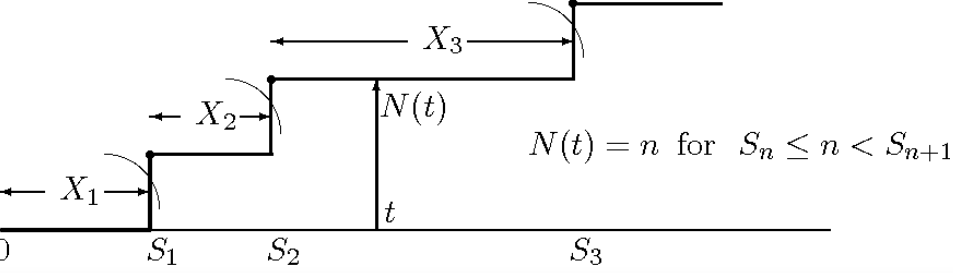
\includegraphics[width=0.5\linewidth, center]{image/arrival_process.png}
\end{figure}
        \begin{itemize}
            \item $X_i$: the time between the $i$-th event and the $i-1$-th event
            \item $S_i$: the time from start to $i$-th event
            \item $N(t)$: the number of the arrived event at time $t$
            \item $X$ and $S$ Relation:
                \begin{itemize}
                    \item $X_1 = S_1, X_i = S_i - S_{i-1}$
                \end{itemize}
            \item $N$ and $S$ Relation:
                \begin{itemize}
                    \item $N(t) < n \leftrightarrow S_{n+1} > t$
                    \item $N(t) \geq n \leftrightarrow S_n \leq t$
                    \item $N(t) = n \leftrightarrow S_n \leq t < S_{n+1}$
                    \item $N(t) = \max \{n: S_n \leq t\}$
                \end{itemize}
            \item Renewal Process: an arrival process with i.i.d $X_i$
                \begin{itemize}
                    \item Delayed Renewal Process: the process becomes a renewal process after $k$ arrivals
                    \item $X_i$ is dependent on the interval states, then $X_i$ might be dependent on $X_{i-1} \rightarrow$ not renewal process
                    \item $\mathbb{E}[X_{N(t) + 1}] \geq \mathbb{E}[X_i]$: inspection paradox
                        \begin{itemize}
                            \item when selecting $t$ with equal probability, we tend to choose $X_i$ with longer period
                        \end{itemize}
                    \item $\mathbb{E}[X_{N(t) + 1}] = \frac{\mathbb{E}[X_i^2]}{\mathbb{E}[X_i]}$
                        \begin{itemize}
                            \item $f_{X_{N(t)+1}}(x) = \lambda x f_{X_i}(x)$
                            \item when selecting $t$ with equal probability, we tend to choose $X_i$ with longer period
                        \end{itemize}
                \end{itemize}
            \item Poisson Process: a renewal process with $X_i \sim \text{Exponential}(\lambda)$

                $S_i$ Property
                \begin{itemize}
                    \item $S_i$ is an Erlang random variable

                        Erlang is the sum of the Exponential random variables
                    \item Joint Distribution $f_{S_1, \dots, S_n}(s_1, \dots, s_n) = \lambda^n e^{-\lambda s_n}$

                        Prove by induction.

                        Induce by $f_{S_1, \dots, S_n}(s_1, \dots, s_n) = f_{S_1, \dots, S_{n-1}}(s_1, \dots, s_{n-1}) \times f_{S_n | S_1, \dots, S_{n-1}}(s_n, s_1, \dots, s_{n-1})$
                \end{itemize}
                $N(t)$ Property
                \begin{itemize}
                    \item $N(t) \sim \text{Poisson}(\lambda t), P[N(t) = n] = \frac{(\lambda t)^n}{n!}e^{-\lambda t}$ 

                        Prove by $P[N(t) = n] = P[S_n \leq t \text{ and } S_{n+1} > t]$
                    \item Conditioned on $N(t) = n$, the set of arrival times $\{s_1, \dots, s_n\}$ have the same distribution with a set of $n$ sorted i.i.d. Uniform$(0, t)$ random variables

                        Prove by $f_{S_1, \dots, S_n | N(t)}(s_1, \dots, s_n, n) = \frac{f_{S_1, \dots, S_n}(s_1, \dots, s_n) P[X_{n+1} > t - s_n]}{P[N(t) = n]} = \frac{n!}{t^n}$
                \end{itemize}
                Property
                \begin{itemize}
                    \item $Z$ is the interval from $t$ to the first arrival $\rightarrow Z$ is exponential random variable with same $\lambda$ and independent of $N(t)$ and the arrival time before $t$

                        Proof:

                        $P[Z > z] = \sum_{n = 0}^\infty \int_0^\infty \dots \int_0^\infty P[Z>z|N(t) = n, S_1 = s_1, \dots, S_n = s_n] ds_1 \dots ds_n$

                        $= \sum_{n = 0}^\infty \int_0^\infty \dots \int_0^\infty P[X_{n+1}>z+t-s_n|N(t) = n, S_1 = s_1, \dots, S_n = s_n] ds_1 \dots ds_n$

                        $= \sum_{n = 0}^\infty \int_0^\infty \dots \int_0^\infty P[X_{n+1}>z+t-s_n|X_{n+1} > t-s_n] ds_1 \dots ds_n = e^{-\lambda z}$
                    \item Stationary Increments: $N(t_1 + t_2) - N(t_1)$ and $N(t_2)$ share the same distribution

                        Without Proof
                    \item Independent Increments: $\forall 0 < t_1 < t_2 < \dots, t_k, N(t_1), N(t_2) - N(t_1), \dots$ are independent

                        Without Proof
                    \item Any arrival process with stationary and independent increments must be a Poisson process

                        Without Proof
                \end{itemize}
                Exercise
                \begin{itemize}
                    \item $\mathbb{E}[S_i|N(t) = n] = \frac{t \times i}{n+1}$
                        \begin{itemize}
                            \item $\mathbb{E}[S_i|N(t) = n] = i \times \mathbb{E}[X_1|N(t) = n] = i \int_0^t \int_0^{s_n} \dots \int_0^{s_2} s_1 \times \frac{n!}{t^n} ds_1 \dots ds_{n-1} ds_n = \frac{t \times i}{n+1}$
                        \end{itemize}
                    \item $\mathbb{E}[\sum_{i=0}^{N(t)} S_i] = \frac{\lambda t^2}{2}$
                        \begin{itemize}
                            \item $\mathbb{E}[\sum_{i=0}^{N(t)} S_i] = \sum_{n = 0}^\infty \mathbb{E}[\sum_{i=0}^n S_i|N(t) = n]P[N(t) = n]$

                                $= \sum_{n = 0}^\infty \frac{nt}{2}P[N(t) = n] = \frac{\lambda t^2}{2}$
                        \end{itemize}
                \end{itemize}
                2D Poisson Process
                \begin{itemize}
                    \item Definition:
                        \begin{itemize}
                            \item For any region $R$: number of points in $R$ is a Poisson random variable
                            \item number of points in the non-overlapping region is independent
                        \end{itemize}
                \end{itemize}
                Combining Poisson Process
                \begin{itemize}
                    \item $N^1(t), N^2(t)$ are two independent Poisson process with $\lambda_1, \lambda_2$
                    \item $X_i$ is the first arrival of $X_i^1, X_i^2$
                    \item Property
                        \begin{itemize}
                            \item $X_i$ is independent of $\{X_i^1 < X_i^2\}$ and $\{X_i^1 > X_i^2\}$ 

                                Proof: $P[X_1^1 < X_1^2] = \frac{\lambda_1}{\lambda_1 + \lambda_2}$

                                $P[X_1 > x] = P[X_1^1 > x, X_1^2 > x] = e^{-(\lambda_1 + \lambda_2)x}$

                                $P[X_1 > x, X_1^1 < X_1^2] = P[X_1 > x]P[X_1^1 < X_1^2]$
                            \item $X_i$ is a Poisson Process with $\lambda = \lambda_1 + \lambda_2$
                        \end{itemize}
                \end{itemize}
                Splitting Poisson Process
                \begin{itemize}
                    \item $N^1(t), N^2(t)$ are two independent Poisson process with $\lambda_1, \lambda_2$
                    \item $N(t)$ is a random process with $\lambda = \lambda_1 + \lambda_2$
                        \begin{itemize}
                            \item $N^{1*}(t)$ is the process of the first event

                                when $N(t)$ arrives consider it as first event with probability $\frac{\lambda_1}{\lambda_1 + \lambda_2}$
                            \item $N^{2*}(t)$ is the process of the second event

                                when $N(t)$ arrives consider it as second event with probability $\frac{\lambda_2}{\lambda_1 + \lambda_2}$
                        \end{itemize}
                    \item $N^i(t)$ and $N^{i*}(t)$ share the same distribution
                    \item Proof:
                        \begin{itemize}
                            \item $B_n(k)$ is a Binomial random variable with $p = \frac{\lambda_1}{\lambda_1 + \lambda_2}$
                            \item $P[N^{1*}(t) = m, N^{2*}(t) = n] = P[N(t) = m + n, B_{m+n}(m)] = P[N^1(t) = m, N^2(t) = n]$
                        \end{itemize}
                \end{itemize}
                Compound Poisson Process
                \begin{itemize}
                    \item $N(t)$ is a Poisson Process
                    \item $A_n$ is a sequence of cost
                    \item $A(t) = \sum_{n=0}^{N(t)} A_n$ is the summation of cost over Poisson Process
                \end{itemize}
        \end{itemize}
\end{itemize}

\end{document}
